\documentclass[]{article}
\usepackage{lmodern}
\usepackage{amssymb,amsmath}
\usepackage{ifxetex,ifluatex}
\usepackage{fixltx2e} % provides \textsubscript
\ifnum 0\ifxetex 1\fi\ifluatex 1\fi=0 % if pdftex
  \usepackage[T1]{fontenc}
  \usepackage[utf8]{inputenc}
\else % if luatex or xelatex
  \ifxetex
    \usepackage{mathspec}
  \else
    \usepackage{fontspec}
  \fi
  \defaultfontfeatures{Ligatures=TeX,Scale=MatchLowercase}
\fi
% use upquote if available, for straight quotes in verbatim environments
\IfFileExists{upquote.sty}{\usepackage{upquote}}{}
% use microtype if available
\IfFileExists{microtype.sty}{%
\usepackage{microtype}
\UseMicrotypeSet[protrusion]{basicmath} % disable protrusion for tt fonts
}{}
\usepackage[margin=1in]{geometry}
\usepackage{hyperref}
\hypersetup{unicode=true,
            pdftitle={Market basket analysis - documentation},
            pdfborder={0 0 0},
            breaklinks=true}
\urlstyle{same}  % don't use monospace font for urls
\usepackage{graphicx,grffile}
\makeatletter
\def\maxwidth{\ifdim\Gin@nat@width>\linewidth\linewidth\else\Gin@nat@width\fi}
\def\maxheight{\ifdim\Gin@nat@height>\textheight\textheight\else\Gin@nat@height\fi}
\makeatother
% Scale images if necessary, so that they will not overflow the page
% margins by default, and it is still possible to overwrite the defaults
% using explicit options in \includegraphics[width, height, ...]{}
\setkeys{Gin}{width=\maxwidth,height=\maxheight,keepaspectratio}
\IfFileExists{parskip.sty}{%
\usepackage{parskip}
}{% else
\setlength{\parindent}{0pt}
\setlength{\parskip}{6pt plus 2pt minus 1pt}
}
\setlength{\emergencystretch}{3em}  % prevent overfull lines
\providecommand{\tightlist}{%
  \setlength{\itemsep}{0pt}\setlength{\parskip}{0pt}}
\setcounter{secnumdepth}{0}
% Redefines (sub)paragraphs to behave more like sections
\ifx\paragraph\undefined\else
\let\oldparagraph\paragraph
\renewcommand{\paragraph}[1]{\oldparagraph{#1}\mbox{}}
\fi
\ifx\subparagraph\undefined\else
\let\oldsubparagraph\subparagraph
\renewcommand{\subparagraph}[1]{\oldsubparagraph{#1}\mbox{}}
\fi

%%% Use protect on footnotes to avoid problems with footnotes in titles
\let\rmarkdownfootnote\footnote%
\def\footnote{\protect\rmarkdownfootnote}

%%% Change title format to be more compact
\usepackage{titling}

% Create subtitle command for use in maketitle
\providecommand{\subtitle}[1]{
  \posttitle{
    \begin{center}\large#1\end{center}
    }
}

\setlength{\droptitle}{-2em}

  \title{\textbf{Market basket analysis - documentation}}
    \pretitle{\vspace{\droptitle}\centering\huge}
  \posttitle{\par}
  \subtitle{Team: Elias and Paul}
  \author{}
    \preauthor{}\postauthor{}
      \predate{\centering\large\emph}
  \postdate{\par}
    \date{2019-07-25}


\begin{document}
\maketitle

\hypertarget{executive-summary}{%
\section{Executive summary}\label{executive-summary}}

\textbf{1. Scope and background}

Blackwell are exploring the possibility of acquiring Electronidex (the
``Target''), an online electronics retailer. The Target has been
presented to us as an enterprise in the start-up stage. We do not have
any information of in which stage of the start-up cycle (e.g.~pre-seed,
seed, seed plus, series A) the Target is currently.

For the purposes of evaluating the feasibility of the transaction, we
have been requested to analyse the Targets sales based on a dataset
containing transactional data about the Targets sales during a period of
30 days. Blackwell has specifically requested that we conduct a
data-mining operation with the purpose of extracting associations
between the different products sold in the transactions in the dataset.
We do not know which month nor have we been furnished such other
information that would allow us to assess, weight or adjust our
conclusions for effects of possible seasonality.

Furthermore, the underlying rationale for the envisioned transaction has
not been disclosed to us. We are assuming that the transaction is
intended as a strategic rather than a financial transaction, but we have
not been made aware what the sought-after addition to the strategic
capability of Blackwell is. Without knowing whether Blackwell is
interested in, for instance, the Targets IP, inorganic growth of
market-share, absolute volume or possible operational synergies
(e.g.~marketing synergy, infrastructure synergy, distribution synergy,
financial advantages), we lack an adequate backdrop against which we
could assess the strategic fit.

We have, however, conducted our review around the hypothesis that
Blackwell is seeking to increase its online presence by acquiring the
Target as a going concern. We have not been made aware of whether
Blackwell intends to merge the Target or its operations into Blackwell
or to keep operating the Target as a stand-alone entity post-closing.

We are not aware of the envisioned deal structure (share or business
purchase, size of stake, leveraged or unleveraged etc.), mode of payment
(cash, shares, mix etc), financials of the Target, financials of
Blackwell, valuation of the Target or a possible integration plan.

Owing to the lack of essential information, we presume that this review
is intended as a part of the limited business review conducted as part
of the initial screening in the acquisition process.

The goal of the initial screening is to assess the overall feasibility
of the acquisition without incurring heavy costs. We have decided to
focus on the part of the so-called 5M (Management, Market, Market-share,
Margins, Model) that the dataset and other provided information allows
us to address in a meaningful way. We lack information that would allow
us to adequately assess the capabilities of the current management, the
prevailing market conditions in the Target's focus market or the
Target's share of any given market.

Consequently, our analysis has focused on trying to gain some form of
superficial understanding of whether there are significant overlaps or
synergies between selections and cross-selling opportunities. The
insights regarding said three subjects can allow us to formulate
hypotheses about some aspects of the Target's business model and margins
that will need to be reviewed and verified in the due diligence stages
of the transaction, should Blackwell decide to progress the transaction
beyond the initial screening phase.

We stress that we are not familiar with the business-model related
items, such as which terms that the Target applies in its supply chain,
we do not know if it operates on the basis of consignment or if they
carry the risk for the inventory, we do not know if the shipping costs
are borne by the customer or the Target, if the Target owns or leases
its warehouses. We are furthermore not aware if the Target is an agency,
distributor or dealer of the brands that it is purveying.

\textbf{2. Associations}

We have in our review prioritised such associations that appear
frequently (in relative terms) in the dataset. In technical terms, we
have used support as the prevailing criterium at the expense of both
lift and confidence.

The rationale for this course of action is the following:

\begin{enumerate}
\def\labelenumi{\roman{enumi})}
\tightlist
\item
  The more frequent an itemset is, the more people we can reach with
  cross-selling efforts;
\item
  The cost of a recommendation (for instance) is low, so one can make as
  many recommendations as deemed appropriate, which decreases the
  importance of the relative ``hit rate'' of an individual
  recommendation;
\item
  For the purposes of an acquisition, we deemed it more relevant to know
  which association rules concerned the largest volume of transactions,
  rather than what the strongest hit rates were because this review was
  based only on a month worth of data, and a larger volume typically
  implies a better representativeness of a sample.
\end{enumerate}

For the purposes of our evaluation, we split out review into five
different reviews. The details of each review are presented in the
appended technical report. We shall only present the conclusions herein.

\begin{enumerate}
\def\labelenumi{\arabic{enumi}.}
\tightlist
\item
  Review of associations within B2B sales:
\end{enumerate}

\begin{itemize}
\tightlist
\item
  No particularly strong rules
\item
  The trend was that Dell and Apple products were often sold together
\item
  This can be a result of the fact that the companies formally buy the
  products but the end-users are the ones deciding what to buy, and
  because preferences vary from one individual to another, we are going
  to see a mix of brands in the basket in B2B sales.
\end{itemize}

\begin{enumerate}
\def\labelenumi{\arabic{enumi}.}
\setcounter{enumi}{1}
\tightlist
\item
  Review of associations within B2C sales:
\end{enumerate}

\begin{itemize}
\tightlist
\item
  No strong rules
\item
  Here we could spot brand preference: Apple products were often
  purchased together with other Apple products
\end{itemize}

\begin{enumerate}
\def\labelenumi{\arabic{enumi}.}
\setcounter{enumi}{2}
\tightlist
\item
  Review of associations between brands:
\end{enumerate}

\begin{itemize}
\tightlist
\item
  Dell and Apple were often purchased together as explained in the B2B
  section
\end{itemize}

\begin{enumerate}
\def\labelenumi{\arabic{enumi}.}
\setcounter{enumi}{3}
\tightlist
\item
  Review of associations between product categories:
\end{enumerate}

\begin{itemize}
\tightlist
\item
  Headphones were often purchased together with laptops
\end{itemize}

\begin{enumerate}
\def\labelenumi{\arabic{enumi}.}
\setcounter{enumi}{4}
\tightlist
\item
  Review of associations between individual products:
\end{enumerate}

\begin{itemize}
\tightlist
\item
  No strong rules
\item
  Dell products were often purchased together with Apple products
\end{itemize}

\textbf{3. Feasibility of acquisition}

As indicated earlier, we lack essential information needed to
appropriately assess the merit of the transaction.

Based on the limited review, it would seem as though the Target has
established a B2B clientele that Blackwell lacks. Acquiring the Target
could be a way to gain that presence.

It would also seem that the Target shows strong sales figures relative
to those of Blackwell in regard of laptops and desktops. We suspect that
this is an effect of the B2B sales, but cannot verify this.

Our recommendation is to progress to the following stage of the
acquisition process, namely the Phase I due diligence after which we
should be better equipped to determine the strategic fit of the Target.

\hypertarget{technical-documentation}{%
\section{Technical documentation}\label{technical-documentation}}

\textbf{Table of contents}\\
1.
\protect\hyperlink{Explorationux5cux2520andux5cux2520preparationux5cux2520ofux5cux2520data}{Exploration
and preparation of data}\\
2. \protect\hyperlink{Comparison}{Comparison of product portfolio}\\
3. \protect\hyperlink{Customerux5cux2520segments}{Analysis on customer
segments (B2C, B2B)}\\
4. \protect\hyperlink{Associationux5cux2520rules}{Association rules
mining}\\
5. \protect\hyperlink{Selectionux5cux2520ofux5cux2520rules}{Selection of
rules}

\hypertarget{exploration-and-preparation-of-data}{%
\subsection{1. Exploration and preparation of
data}\label{exploration-and-preparation-of-data}}

The transaction set contains \emph{9835} transactions. The average
transaction size contains \emph{4.38271479410269} items.

Plotting the frequency of products purchased in all transactions one can
see from the figure below that iMac is the top-selling product for
Electronidex followed by HP Laptop and CYBERPOWER Gamer Desktop. Amongst
top 5 there are additionally two other Apple products, namly Earpods and
MacBook Air.

\begin{center}\includegraphics{MBA_files/figure-latex/unnamed-chunk-2-1} \end{center}

The following graph visualizes a random sample of the underlying
transaction data. Using this depiction, there are apparently no patterns
to be observed.

\begin{center}\includegraphics{MBA_files/figure-latex/Image-1} \end{center}

\hypertarget{comparison-of-product-portfolio}{%
\subsection{2. Comparison of product
portfolio}\label{comparison-of-product-portfolio}}

To compare the product portfolios of both companies the selling record
is plotted against main product categories. One can clearly state that
Blackwell sells a huge amount of Accessories whereas all other
categories besides GameConsole and Software are quite low. In comparison
to that Electronidex holds a huge stack in PC and Laptops. These are
especially considered as strategic selling categories as they over high
cross-selling potential for peripherical product categories, primarily
Accessories and Speakers. Based on this view on product portfolio
synergies could be found with the acquisition as both portoflios
supplement each other in several categories.

\begin{center}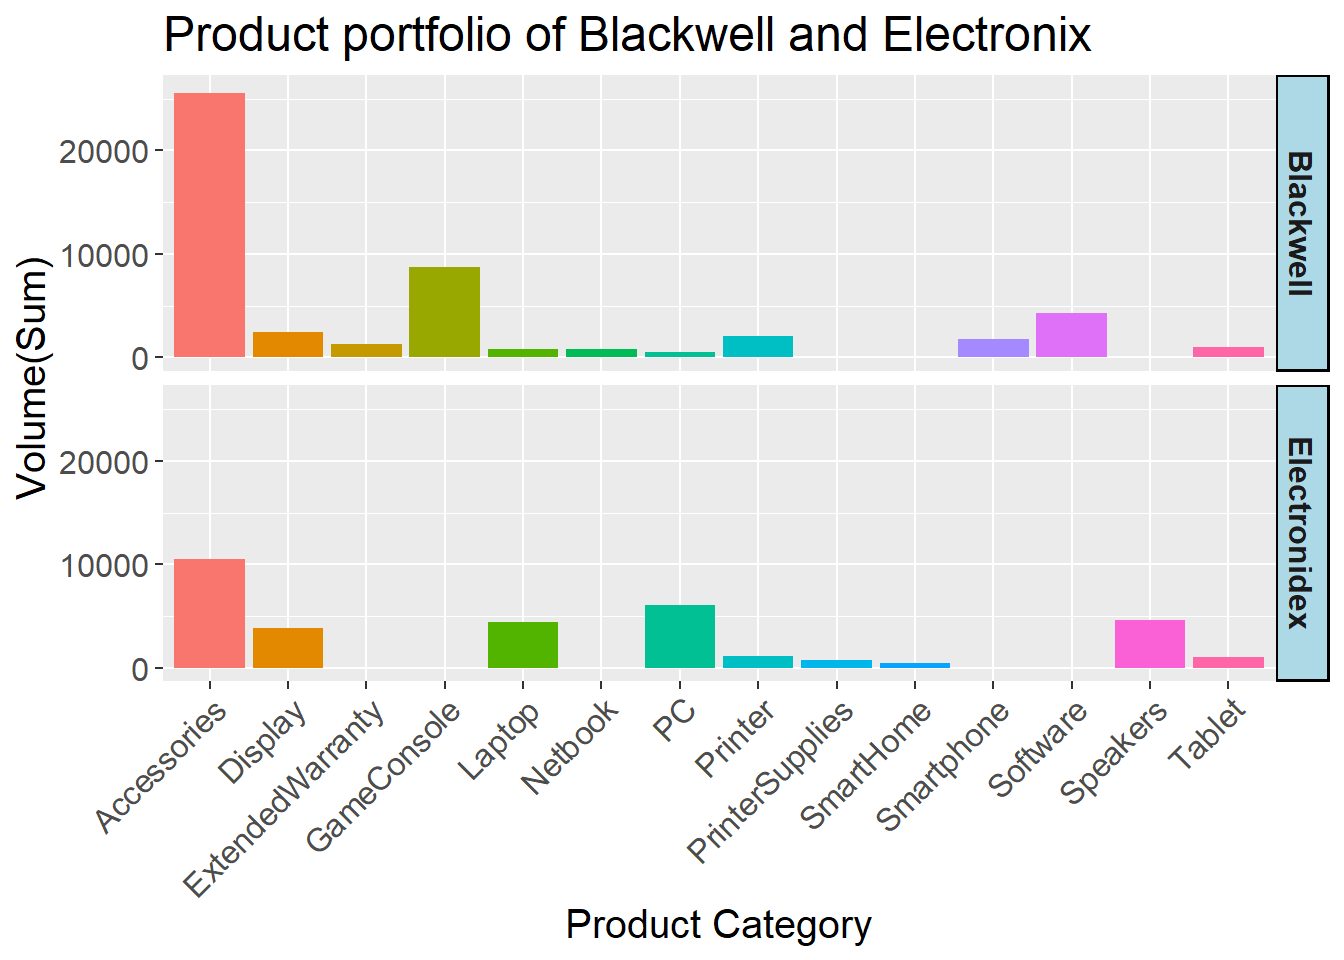
\includegraphics{MBA_files/figure-latex/Portfolio comparison-1} \end{center}

\begin{itemize}
\tightlist
\item
  Accessories contain `Computer Cords', `Computer Stands', `External
  Hardrives', `Keyboard', `Mouse', `Mouse and Keyboard'\\
\item
  Speakers contain `Computer Headphones', `Active Headphones'
\end{itemize}

\hypertarget{analysis-on-customer-segments-b2c-b2b}{%
\subsection{3. Analysis on customer segments (B2C,
B2B)}\label{analysis-on-customer-segments-b2c-b2b}}

To revail patterns for different customer segments, i.e.~B2C and B2B,
the transaction dataset has been splitted. This seemed to be meaningful
in terms of getting insights on customer buying patterns in relation to
certain valueable products (i.e.~PC and Laptop), transaction size.
Besides this the cluster takes Printer and Monitor into account as they
are frequently used in business environments and thus considered to be a
good indicator. As the data gives no information on customer segment the
split has been done using predefined cut values. These cut values are
found in a previous cluster analysis applying kmeans cluster algorithm.

\begin{center}\includegraphics{MBA_files/figure-latex/Visualization of cluster analysis-1} \end{center}

\begin{center}\includegraphics{MBA_files/figure-latex/Visualization of cluster analysis-2} \end{center}

\begin{center}\includegraphics{MBA_files/figure-latex/Visualization of cluster analysis-3} \end{center}

\begin{center}\includegraphics{MBA_files/figure-latex/Visualization of cluster analysis-4} \end{center}

The transactions has been splitted using the cut values found by the use
of Cluster analysis. This leads to a total number of transactions in the
B2C segment of \emph{5073}, whereas \emph{4762} has been refered to the
B2B segment.

The item frequency plots reveal the preferred products for consumers and
business customers.

\begin{center}\includegraphics{MBA_files/figure-latex/itemFrequ for b2c b2b-1} \end{center}

\begin{center}\includegraphics{MBA_files/figure-latex/itemFrequ for b2c b2b-2} \end{center}

\hypertarget{association-rules-mining}{%
\subsection{4. Association rules
mining}\label{association-rules-mining}}

\begin{center}\includegraphics{MBA_files/figure-latex/Visualization - Scatter-1} \end{center}

\begin{center}\includegraphics{MBA_files/figure-latex/Visualization - Scatter-2} \end{center}

\begin{center}\includegraphics{MBA_files/figure-latex/Visualization - Scatter-3} \end{center}

\begin{center}\includegraphics{MBA_files/figure-latex/Visualization - Scatter-4} \end{center}

\begin{center}\includegraphics{MBA_files/figure-latex/Visualization - Scatter-5} \end{center}

\hypertarget{selection-of-rules}{%
\subsection{5. Selection of rules}\label{selection-of-rules}}

\includegraphics{MBA_files/figure-latex/Visualization - Rules graphs-1.pdf}
\includegraphics{MBA_files/figure-latex/Visualization - Rules graphs-2.pdf}
\includegraphics{MBA_files/figure-latex/Visualization - Rules graphs-3.pdf}
\includegraphics{MBA_files/figure-latex/Visualization - Rules graphs-4.pdf}
\includegraphics{MBA_files/figure-latex/Visualization - Rules graphs-5.pdf}


\end{document}
